\chapter{Spin models of many-body systems}
\label{ch:systems}

After the general introduction in the previous chapter, we now provide the formal definitions of the physical systems studied in this thesis, along with the motivations to study them. We mainly focus on systems of spin-$\frac{1}{2}$ particles placed on lattices, and most results are generalizable to higher spins, fermions, and bosons. Specifically, we focus on classical systems in thermal equilibrium, and quantum systems at ground states.

\section{Classical systems}
\label{sec:cl-sys}

\subsection{Ising model}
\label{sec:cl-ising}

The early studies of the Ising model~\cite{ising1925contribution, niss2008history} predates the modern formulation of quantum physics. It was proposed to describe the properties of ferromagnets using spins $\vs = (s_1, s_2, \ldots, s_N)$ on a lattice of $N$ sites, where each spin $s_i$ can take the values $\pm 1$, so the Hamiltonian function of the system is
\begin{equation}
H(\vs) = J \sum_{\langle i, j \rangle} s_i s_j,
\label{eq:cl-ising}
\end{equation}
where $\langle i, j \rangle$ runs over nearest neighbors on the lattice. We omit the external fields for simplicity, and we assume $J = 1$ unless otherwise stated. When the system is in thermal equilibrium at the temperature $T$, or more conventionally the inverse temperature $\beta = \frac{1}{T}$, it is described by an ensemble of spin configurations following the Boltzmann distribution
\begin{align}
p_\text{B}(\vs) &= \frac{\rme^{-\beta H(\vs)}}{Z}, \label{eq:boltzmann} \\
Z &= \sum_\vs \rme^{-\beta H(\vs)},
\end{align}
where $Z$ is called the partition function.

While the Curie--Weiss mean-field theory~\cite{weiss1907hypothese} predicted a second-order phase transition at the critical point $\beta_\text{c} = \frac{1}{2 D}$, where $D$ is the spatial dimension, the analytical solutions established that there is no phase transition in one dimension (1D)~\cite{ising1925contribution}, a second-order phase transition in the thermodynamic limit on two-dimensional (2D) grids at $\beta_\text{c} = \frac{1}{2} \ln(1 + \sqrt{2}) \approx 0.44$~\cite{onsager1944crystal}, as well as second-order phase transitions on four- and higher-dimensional grids where the mean-field theory is asymptotically exact~\cite{als1977mean}. However, no analytical solution in three dimensions (3D) is known yet~\cite{viswanathan2022does}.

Although the above formulation of spins is too simplified in the viewpoint of quantum physics, the Ising model revived in the studies of various quantum systems, as we will see in \cref{sec:qu-ising}, notably being the simplest model for quantum phase transitions~\cite{sachdev2001quantum}. The classical formulation is still relevant when the quantum hopping effect described by the transverse field is negligible. With the presence of the transverse field, it has also been shown that any quantum Ising model in $D$ dimensions can be mapped to a classical one in $D + 1$ dimensions in the same universality class~\cite{hertz1976quantum}, which opens a practical way to study these quantum systems. Moreover, the same mathematical form appears in the tight-binding theory of electronic bands~\cite{treglia1988segregation}.

\subsection{Observables}

Given the distribution of the configurations $p(\vs)$, we can obtain the macroscopic expectation value of any physical observable $O(\vs)$ by
\begin{equation}
\bar{O} = \sum_\vs p(\vs) O(\vs).
\label{eq:cl-obs}
\end{equation}
The observables of common interest include the energy $E$, the heat capacity $\calC_V$, the magnetization $M$, the magnetic susceptibility $\chi_M$, and the spin correlation $C(d)$ as a function of the distance $d$. We note that $\calC_V$ and $\chi_M$ can be expressed from the fluctuations of $E$ and $M$ respectively, or alternatively from the derivatives of the partition function. It is also feasible to evaluate the entropy
\begin{equation}
S = -\sum_\vs p(\vs) \ln p(\vs)
\end{equation}
and the free energy
\begin{equation}
F = -T \ln Z = E - T S,
\end{equation}
which require to evaluate the partition function itself in $\ln p(\vs)$, and lead to extra difficulty compared to the above observables. Moreover, the ground state and its energy
\begin{align}
\vs_0 &= \arg\min_\vs H(\vs), \\
E_0 &= \lim_{T \to 0} E = H(\vs_0)
\end{align}
are of interest with non-trivial lattice geometries and interactions, which has its root in combinatorial optimization problems in mathematics and computer sciences, as we will discuss in \cref{sec:random-interactions}.

The analytical solutions to these observables are attainable only in some cases of simple lattice geometries and interactions. Many 1D systems are solvable using the transfer matrix method~\cite{chaikin1995principles5}, with a few results in 2D~\cite{baxter1995solvable, march2016exactly, caravelli2022some}. In the remaining cases, which include rich and unknown physical phenomena, numerical methods are required to study them.

However, the efficiency of numerical methods is impeded by the sheer high dimension of the configuration space. The summation in \cref{eq:cl-obs} runs over $2^N$ possible configurations of the system in total, which is exponentially large and quickly becomes intractable as $N$ increases. As of this writing, the largest supercomputers in the world have peak computational power on the order of $10^{18}$ floating-point operations per second ($1$ exaFLOPS)~\cite{kogge2022frontier}, which can sum over only $81$ spins in the ``sane'' time budget of a month, even if the summation is unrealistically optimized to take one floating-point operation for each configuration, and other costs such as the storage are ignored. This means we can only resort to approximation methods to compute the expectation in practice, which we will discuss in the following chapters.

\subsection{Geometrical frustration and residual entropy}
\label{sec:frustrate}

A difficulty in solving the Ising model comes from the lattice geometry, as shown in \cref{fig:frustrate}. If the system is ferromagnetic (FM) with $J < 0$ in \cref{eq:cl-ising}, where every pair of interacting spins tend to align in the same direction to produce lower energy, then the ground state is intuitively obtained when all spins are aligned. On the contrary, if the system is antiferromagnetic (AFM) with $J > 0$, and the lattice contains odd-length cycles, then there is no longer an intuitive way to obtain the ground state, and even a simple system of three spins has as many as six degenerate ground states. This phenomenon is known as the geometrical frustration.

\begin{figure}[htb]
\centering
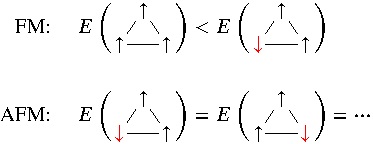
\includegraphics[width=0.5\linewidth]{ch2/frustrate.pdf}
\caption[Frustrated interactions in Ising model]{
The non-frustrated FM and the frustrated AFM interactions for the Ising model on a triangle of three spins.
}
\label{fig:frustrate}
\end{figure}

On a triangular lattice of $N$ spins, the number of degenerate ground states $N_\text{GS}$ grows exponentially with $N$, which poses challenge for analytical and numerical methods to accurately evaluate the observables, or merely count the order of magnitude of $N_\text{GS}$. Besides the triangular lattice~\cite{liu2020intrinsic}, other kinds of frustrated lattices also appear in the modeling of materials, such as the kagome lattice~\cite{wolf1988ising} and the pyrochlore (tetrahedral) lattice~\cite{siddharthan1999ising}. The disordered ground states can lead to the spin liquid phase in the quantum description of these materials, which is an active topic of research.

At zero temperature, only the ground states contribute to the entropy:
\begin{equation}
\lim_{\beta \to \infty} S = \ln N_\text{GS}.
\end{equation}
In the thermodynamic limit $N \to \infty$, we assume
\begin{equation}
N_\text{GS} = A \rme^{c N},
\end{equation}
where $A$ and $c$ are coefficients to be determined. Then we have
\begin{equation}
\lim_{\beta \to \infty} \frac{S}{N} = \frac{\ln A}{N} + c,
\end{equation}
which converges to $c$ as $N \to \infty$, and $c$ is known as the residual entropy~\cite{wannier1950antiferromagnetism, mambrini1999residual, vanderstraeten2018residual}. The existence of a non-zero residual entropy indicates the exponentially large number of degenerate ground states. For the relatively simple case of Ising model on the 2D triangular lattice, the analytical result has been derived~\cite{wannier1950antiferromagnetism, wannier1973antiferromagnetism}:
\begin{equation}
\lim_{N \to \infty} \lim_{\beta \to \infty} \frac{S}{N} = \frac{2}{\pi} \int_0^{\frac{\pi}{3}} \ln(2 \cos \omega) \dd \omega \approx 0.323.
\end{equation}
This residual entropy will be studied in \cref{sec:arnn-tri-ising}. In addition, we mention that the boundary conditions of finite-sized systems can substantially affect the observables in the presence of frustration.

\subsection{Spin glass}
\label{sec:random-interactions}
\label{sec:ea}
\label{sec:sk}

Besides the geometrical frustration, another cause of disorder in Ising models is that the interactions $J_{i j}$ between the spins can be random. In this case, the Hamiltonian function is written as
\begin{equation}
H(\vs) = \sum_{i j} J_{i j} s_i s_j.
\label{eq:cl-ising-general}
\end{equation}
This kind of systems are known as spin glasses~\cite{fischer1993spin, nishimori2001statistical}, because of the analogy to the positional disorder in conventional amorphous glasses. The random interactions can produce numerous metastable states, which makes it difficult to investigate the properties around the true ground state. Even with the optimization power of nature, the spin glass materials actually have long relaxation times to reach the equilibrium.

In particular, the Sherrington--Kirkpatrick (SK) model~\cite{sherrington1975solvable} is an early example of spin classes. It is defined for $N$ spins interacting with each other, and each interaction strength $J_{i j}$ is sampled from a Gaussian distribution with zero mean and a variance of $\frac{1}{N}$. The Edwards--Anderson (EA) model~\cite{edwards1975theory} is another example, which is defined on a lattice with nearest-neighbor interactions:
\begin{equation}
H(\vs) = J \sum_{\langle i, j \rangle} J_{i j} s_i s_j.
\end{equation}
The interaction strength $J_{i j}$ is conventionally sampled from a Gaussian distribution, and in \cref{sec:twobo-results} we will study a variant with binary interactions, where each $J_{i j}$ randomly takes $\pm 1$. In the limit of large system size with the average over random interactions, they can be studied using the replica method~\cite{parisi1979infinite}, while the cases with finite system sizes and specific interactions are still of practical interest.

Besides modeling a variety of non-uniform alloys and compounds~\cite{mydosh2015spin}, spin glasses also appear in the boarder fields of mathematics and computer sciences. Finding the ground state of a spin glass model with specific interactions is equivalent to several combinatorial optimization problems that are known to be hard, such as the quadratic unconstrained binary optimization (QUBO), the maximum cut of graphs (max-cut), and the boolean satisfiability with three literals (3-SAT)~\cite{karp1972reducibility}. In particular, while it has been proven that finding the ground state only has polynomial time complexity on 2D lattices without external fields, it is NP-hard on 2D lattices with external fields, and on 3D lattices~\cite{barahona1982computational}. Moreover, computing the partition function is \#P-hard on general graphs~\cite{galanis2016inapproximability, fefferman2017exact, peters2020location}. Both NP-hard and \#P-hard problems are at least as hard as NP-complete problems, which cannot be solved in polynomial time unless P = NP. This means if we aim to exactly and provably find the ground state or its energy in the general case, then any smart algorithm is unlikely to be substantially faster than the brute-force enumeration. Therefore, we are further motivated to develop non-deterministic and heuristic approximation methods for this kind of problems.

\subsection{Associative memory}
\label{sec:hopfield}

Ising models also manifest in the studies of associative memory, in the sense that we can encode data in its parameters and retrieve the data by sampling from it. This kind of models have their root in both computer sciences and neurosciences~\cite{carpenter1989neural}. An example is the Hopfield model~\cite{hopfield1982neural, amit1985spin}, which we will study in \cref{sec:arnn-hop}. It is defined by the fully connected Ising model in \cref{eq:cl-ising-general} with the interactions
\begin{equation}
J_{i j} = -\frac{1}{N} \sum_{p = 1}^{n_\text{pat}} \xi^{(p)}_i \xi^{(p)}_j,
\label{eq:hopfield}
\end{equation}
where $\{\vxi^{(1)}, \vxi^{(2)}, \ldots, \vxi^{(n_\text{pat})}\}$ are some special spin configurations, known as the ``patterns'', and $n_\text{pat}$ is the number of patterns. The patterns are usually orthogonal:
\begin{equation}
\ip{\vxi^{(p)}}{\vxi^{(q)}} = 0 \quad \forall p, q,
\label{eq:cl-ortho}
\end{equation}
where the overlap between two configurations is defined by
\begin{equation}
\ip{\vs}{\vs'} = \frac{1}{N} \sum_i s_i s'_i.
\label{eq:cl-overlap}
\end{equation}
For any configuration $\vs$ and two orthogonal patterns $\vxi^{(1)}$ and $\vxi^{(2)}$, we have
\begin{equation}
\Big| \ip{\vs}{\vxi^{(1)}} \Big| + \Big| \ip{\vs}{\vxi^{(2)}} \Big| \le 1,
\end{equation}
which will be seen in \cref{fig:arnn-hop}. The model has $2 n_\text{pat}$ degenerate ground states: $\vs_0 = \pm \vxi^{(p)}$, $H(\vs_0) = -N$. Therefore, we say the model ``memorizes'' the patterns.

\subsection{Frustrated plaquette model (FPM)}
\label{sec:fpm}

While the previous models only have second-order phase transitions, one way to produce first-order phase transitions is to include interactions between more spins. We have constructed a frustrated plaquette model (FPM) as an example of first-order phase transition, which we will study in \cref{sec:ncus-fpm}.

The FPM is defined on an $L \times L$ lattice of the spins $s_{x, y}$, with nearest-neighbor $J_1$, third-nearest-neighbor $J_3$, and plaquette $K$ interactions:
\begin{align}
H(\vs) = &\phantom{{}+{}} J_1 \sum_{i, j = 1}^L s_{i, j} (s_{i + 1, j} + s_{i, j + 1})
+ J_3 \sum_{i, j = 1}^L s_{i, j} (s_{i + 2, j} + s_{i, j + 2}) \nonumber \\
&+ K \sum_{i, j = 1}^L s_{i, j} \, s_{i + 1, j} \, s_{i, j + 1} \, s_{i + 1, j + 1}.
\label{eq:fpm}
\end{align}
When $J_1 = J_3 = -1$, its phase diagram with varying $K$ and $T$ is shown in \cref{fig:fpm-phase}. Besides the paramagnetic (PM) phase at high $T$, it has a ferromagnetic (FM) phase at low $T$ and low $K$, and a ferrimagnetic (fM) phase at low $T$ and high $K$. In the fM phase, the ground state breaks the spin-inversion symmetry and the one-site translational symmetry, which is the result of the competing $J_1$, $J_3$, and $K$ interactions.

\begin{figure}[htb]
\centering
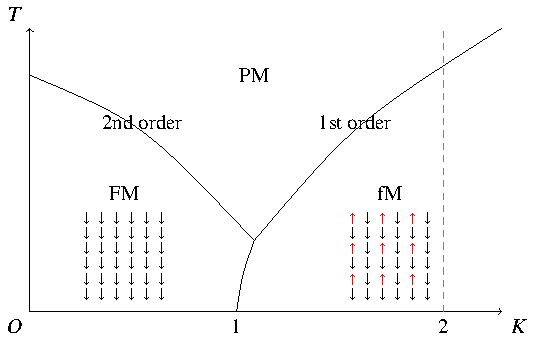
\includegraphics[width=0.7\linewidth]{ch2/fpm_phase.pdf}
\caption[Phase diagram of frustrated plaquette model (FPM)]{
Sketch of the phase diagram for the FPM with varying plaquette interaction strength $K$ and temperature $T$, at $J_1 = J_3 = -1$.
Examples of the ground state in the ferromagnetic (FM) and the ferrimagnetic (fM) phases are shown respectively.
The case of $K = 2$ as indicated by the dashed vertical line is studied in Ref.~\cite{wu2021unbiased}, with a first-order phase transition between the fM and the paramagnetic (PM) phases.
This figure is reproduced from Fig.~3~(a) in Ref.~\cite{wu2021unbiased}.
}
\label{fig:fpm-phase}
\end{figure}

Although not covered by our research, it is worth mentioning that the Wishart planted ensemble~\cite{hamze2020wishart, hibat2021variational} has been proposed to be a more controllable example of first-order phase transition, as well as a more modern example of associative memory.

\section{Quantum systems}
\label{sec:qu-sys}

\subsection{Heisenberg model}

The Heisenberg model~\cite{heisenberg1928theorie} is a common description for the magnetic properties of materials in quantum physics. It assumes that the electrons are localized on the lattice, so the energy levels are only determined by their spin interactions, rather than positional interactions. The Hamiltonian is written as
\begin{equation}
\hat{H} = J \sum_{\langle i, j \rangle} \hat{\vsi}_i \cdot \hat{\vsi}_j,
\label{eq:heis}
\end{equation}
where the Pauli operators for spin-$\frac{1}{2}$ particles are represented by
\begin{equation}
\hat{\sigma}^x = \begin{pmatrix} 0 & 1 \\ 1 & 0 \end{pmatrix}, \quad
\hat{\sigma}^y = \begin{pmatrix} 0 & -i \\ i & 0 \end{pmatrix}, \quad
\hat{\sigma}^z = \begin{pmatrix} 1 & 0 \\ 0 & -1 \end{pmatrix},
\end{equation}
and $\hat{\vsi}_i \cdot \hat{\vsi}_j = \hat{\sigma}^x_i \hat{\sigma}^x_j + \hat{\sigma}^y_i \hat{\sigma}^y_j + \hat{\sigma}^z_i \hat{\sigma}^z_j$ is the dot product of two 3D vectors of Pauli operators. It can also be derived from the Hubbard model with half filling of electrons and small hopping strength, where in the ground state each site is occupied by an electron, and the electron exchanges are given by the second order perturbation of hopping~\cite{cleveland1976obtaining}.

The ground state of the system is determined by
\begin{equation}
\ket{\psi_0} = \arg\min_{\ket{\psi}} \ev{\hat{H}}{\psi},
\label{eq:gs}
\end{equation}
which contains the complete information about the system at zero temperature, and is usually the foundation for further studying the excitations or the thermal properties of the system. In contrast to the classical case, even if the quantum system is at the ground state and is non-degenerate, it can still be a superposition of exponentially many basis states $\ket{\vs}$. Given a state $\ket{\psi}$, we can obtain the expectation value of any physical observable $\hat{O}$ by
\begin{equation}
\bar{O} = \ev{\hat{O}}{\psi} = \sum_{\vs, \vs'} \psi^*(\vs) O(\vs, \vs') \psi(\vs),
\label{eq:qu-obs}
\end{equation}
where $\psi(\vs) = \ip{\vs}{\psi}$ and $O(\vs, \vs') = \mel{\vs}{\hat{O}}{\vs'}$. Same as the classical case, the summation in \cref{eq:qu-obs} also contains exponentially many terms and is intractable. Worse still, to exactly compute the ground state vector in \cref{eq:gs} in general, one needs the exact diagonalization (ED) of the $2^N \times 2^N$ Hamiltonian matrix, which takes even higher exponential time~\cite{weisse2008exact}. Therefore, we again need approximation methods to study the system in practice.

The issue of frustration discussed in \cref{sec:frustrate} also occurs in the quantum case. On frustrated lattices such as the triangular lattice~\cite{li2015rare}, the kagome lattice~\cite{norman2016colloquium} and the pyrochlore lattice~\cite{moessner1998properties}, the Heisenberg model can exhibit spin liquid phases. Another model commonly believed to exhibit the spin liquid phase is the $J_1$-$J_2$ model, which is defined as the Heisenberg model with next-nearest-neighbor interactions~\cite{dagotto1989phase, schulz1996magnetic, hu2013direct, liu2018gapless}.

% QMA-complete~\cite{troyer2005computational, kempe2006complexity, oliveira2008complexity}

\subsection{Transverse-field Ising model (TFIM)}
\label{sec:qu-ising}

The transverse-field Ising model (TFIM) is formulated as the classical Ising model in \cref{sec:cl-ising} with a transverse field $\Gamma$ describing the quantum hopping effect. Its Hamiltonian is written as
\begin{equation}
\hat{H} = J \sum_{\langle i, j \rangle} \hat{\sigma}^z_i \hat{\sigma}^z_j
+ \Gamma \sum_i \hat{\sigma}^x_i.
\label{eq:qu-ising}
\end{equation}
Its usages in the early days of solid-state physics include a special case of anisotropic Heisenberg model~\cite{katsura1962statistical}, and a phenomenological model with fictitious spins, such as the order-disorder transition of the ferroelectric crystal KH$_2$PO$_4$~\cite{de1963collective}. With deeper research into the classification of phase transitions, it has been known as the simplest model to demonstrate the quantum phase transition at zero temperature, which is driven by quantum fluctuations rather than thermal fluctuations~\cite{sachdev2001quantum, suzuki2012quantum}. This actually describes the phase transitions of several magnetic materials, such as LiHOF$_4$~\cite{bitko1996quantum} and CoNb$_2$O$_6$~\cite{coldea2010quantum}.

The TFIM in 1D has been analytically solved with the critical point $\Gamma_\text{c} = 1$. The analytical solution in 2D is unknown yet, which has the same difficulty as the 3D classical Ising model because of the mapping between them, while numerical methods has estimated $\Gamma_\text{c} \approx 3.04438(2)$~\cite{blote2002cluster}.

\subsection{Quantum thermal state}

We also mention that beyond the ground state, a quantum system can be a mixed state described by a density matrix, and represented in the eigenbasis by
\begin{equation}
\hat{\rho} = \sum_i p_i \ket{\psi_i}\bra{\psi_i},
\end{equation}
where $\ket{\psi_i}$ is the $i$-th lowest eigenstate of the Hamiltonian, and $p_i$ is the corresponding probability of measuring this state. When the system is at the temperature $T$ in thermal equilibrium, $p_i$ is given by the Boltzmann distribution. Knowing the density matrix, we can obtain the expectation value of any physical observable $\hat{O}$ by
\begin{equation}
\bar{O} = \tr[\hat{O} \hat{\rho}].
\label{eq:dm-obs}
\end{equation}
The density matrix poses extra difficulties of computing both the states $\left\{ \ket{\psi_i} \right\}$ and their probabilities $\{p_i\}$. In this thesis, we mainly focus on the ground state.
